\chapter{Anomaly Detection}

We may refer to anomalies in data also as \textit{outliers.}

\section{Outliers}
\begin{itemize}
	\item Inherently \textbf{fuzzy} - An instance has a degree of outlierness, which we can threshold to decide whether an instance is an outlier or not.
	\item \textbf{Data-dependent} - Outlier are exceptions to the data. But outliers themselves define the data...?
	\item \textbf{Not noise} - Noise is random, outliers are exceptional.
	\item \textbf{Mono/multi-dimensional} - An outlier can be so on one just one dimension, or on multiple.
\end{itemize}

Outliers are something that is either \textbf{unusual} or \textbf{extreme}, or both.\\
Outliers are, by nature, defined in terms of other instances. Whatever approach we use to detect them, we should take into account that they influence it as well.

\section{Outlier Detection Algorithms}
Algorithms used to detect outliers usually involve two key steps:
\begin{enumerate}
   \item \textbf{Grading} - Define a grading function $\tilde{o}$ that assigns to each instance $x$ a degree of outlierness/anomaly $\tilde{o}(x)$.
   \item \textbf{Thresholding} - Decide on a threshold $\hat{o}$ such that instances with $\tilde{o}(x) > \hat{o}$ are considered outliers.
\end{enumerate}

We can categorize outlier detection algorithms depending on the \textit{axis} on which they operate:
\begin{itemize}
   \item \textbf{Locality} - is the outlier detection performed in a local neighborhood (local) or considering the entire dataset (global)?
   \item \textbf{Sensitivity} - is the outlier detection sensitive to the presence of other outliers (sensitive) or not (robust)?
   \item \textbf{Interpretability} - can we interpret/explain why an instance is considered an outlier (interpretable) or not (black-box)?
\end{itemize}

\begin{table}
   \begin{tabular}{|c|c|}
      \textbf{Locality} & \textbf{Global}/\textbf{Local} \\
      \hline
      \textbf{Sensitive} & \textbf{Robust}/\textbf{Sensitive} \\
      \hline
      \textbf{Interpretable} & \textbf{Black-box}/\textbf{Interpretable} \\
   \end{tabular}
\end{table}

\begin{figure}[htbp]
   \centering
   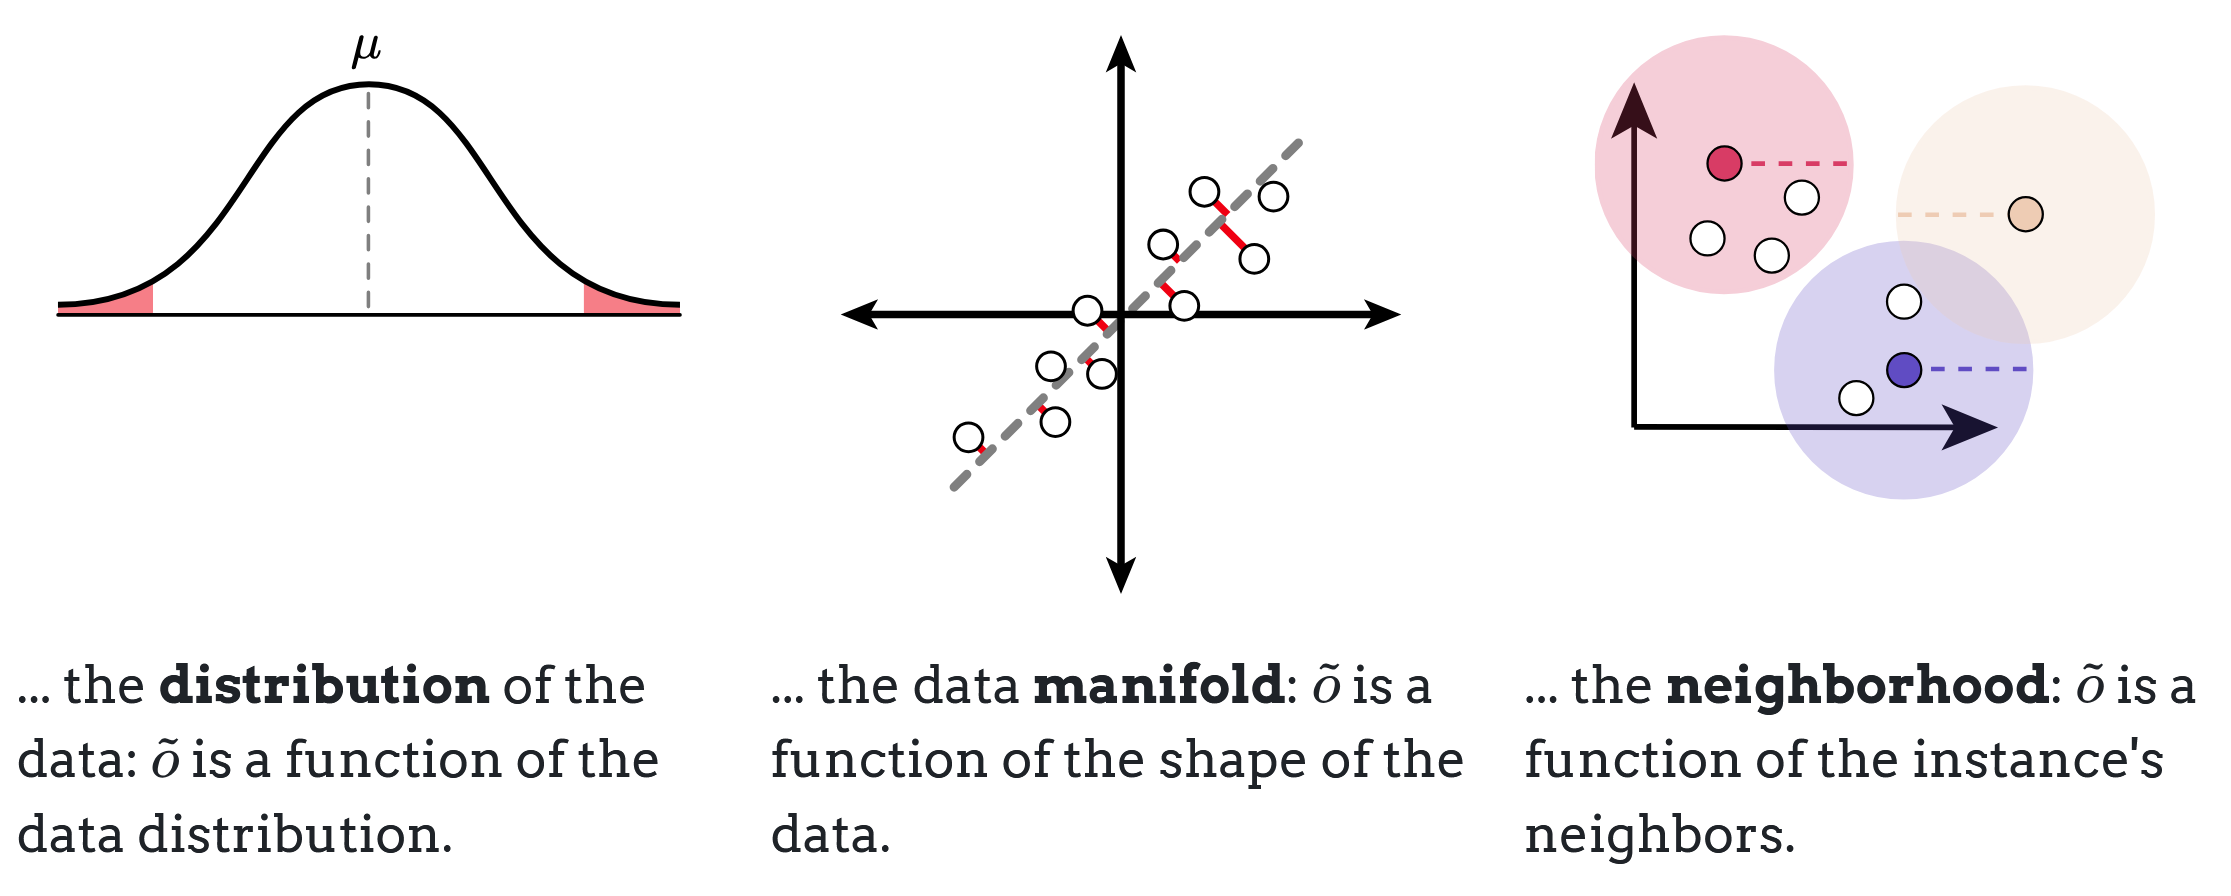
\includegraphics{images/06/outlierfunction}
   \caption{Distribution, manifold, neighborhood}
   \label{fig:}
\end{figure}

\subsection{Distributions}
\begin{paracol}{2}
   In case of a normal distribution $\mathcal{N}(\mu, \sigma)$, we can define outliers as instances that are more than $k$ standard deviations away from the mean $\mu$ (see Figure~\ref{fig:06/normaldistribution}).\\
   This approach is \textbf{global}, \textbf{robust} and \textbf{interpretable}.

   The degree of anomaly $\tilde{o}(x)$ can be defined as:
   \[
      \text{z-score} = \tilde{o}(x) = \frac{|x - \mu|}{\sigma}
   \]

   \switchcolumn

   \begin{figure}[htbp]
      \centering
      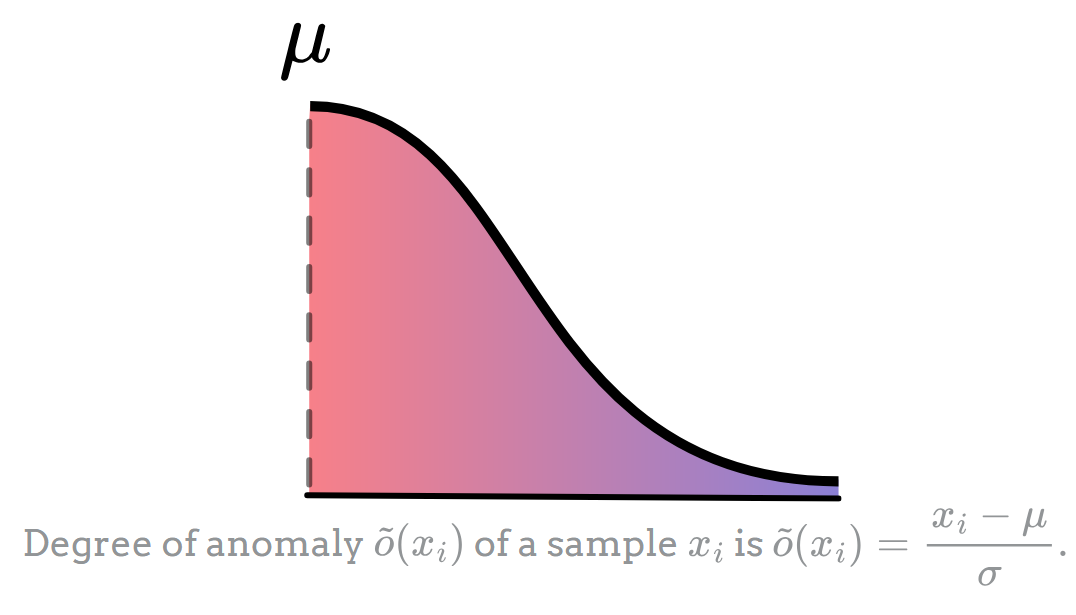
\includegraphics{images/06/normaldistribution.png}
      \caption{For a normal distribution $\mathcal{N}(\mu, \sigma)$, we can define outliers as instances that are more than $k$ standard deviations away from the mean $\mu$.}
      \label{fig:06/normaldistribution}
   \end{figure}
\end{paracol}

\subsubsection{Grubbs test}
$z-scores$ generate sample-dependent outlier degrees $\tilde{o}(x_1), \tilde{o}(x_2), \ldots, \tilde{o}(x_n)$, but does not tackle the \textbf{+1 problem}.

The +1 problem is the problem of deciding whether the most extreme instance in a dataset is an outlier or not.\\
Grubb's test iterates over detected outliers, removing one layer of outliers at a time, until no more outliers are found.
\begin{algorithm}
   \caption{Grubb's test for outliers}
   \begin{algorithmic}[1]
      \State Find current outlier set $\hat{X}$
      \State If $\hat{X} = \emptyset$, stop
      \State $X = X \setminus \hat{X}$ - remove outliers from dataset
      \State Go to step 1
   \end{algorithmic}
\end{algorithm}

\begin{table}
   \begin{tabular}{|c|c|}
      \textbf{Locality} & \textbf{Global} \\
      \hline
      \textbf{Sensitive} & Outliers influence the distribution but may be removed by Grubb's test \\
      \hline
      \textbf{Interpretable} & \textbf{Black-box}, no clear explanation for outlierness, simply, there are not many similar instances.\\
   \end{tabular}
\end{table}


Data may vary \textit{locally}: subsets of the data each follow a different distribution.\\
Assumption: there exists a partition of the data, each block distributed according to a Normal distribution.\\
Thus we could use multiple models to model the data, and define outliers as instances that are outliers with respect to their local distribution.\\

One of $k$ models $M_{\theta_{0}}, M_{\theta_{1}}, \ldots, M_{\theta_{k-1}}$ is sampled, each with a sampling probability $m_i$. Different distributions sample different regions of the density.

\begin{figure}[htbp]
   \centering
   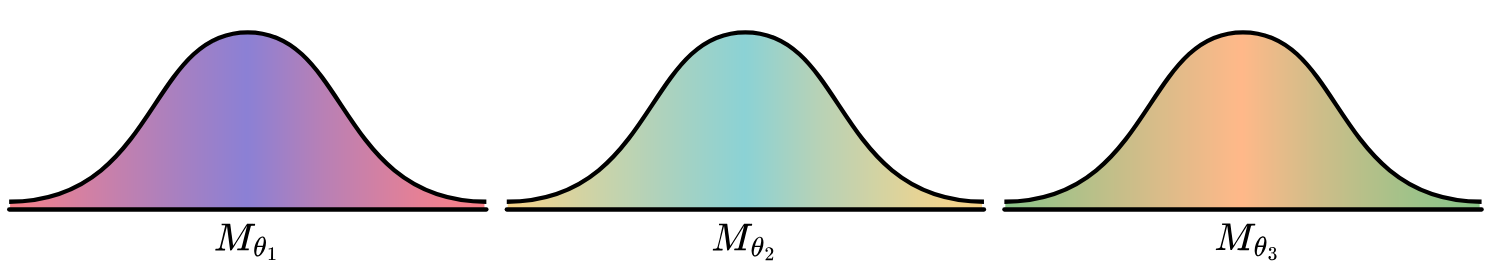
\includegraphics{images/06/mixture.png}
   \caption{A mixture of Normals $M_{\theta_0}, M_{\theta_1}, M_{\theta_2}$; each sampled with probability $m_0, m_1, m_2$, respectively.}
   \label{fig:06/mixture}
\end{figure}

\begin{table}
   \begin{tabular}{|c|c|}
      \textbf{Locality} & \textbf{Local} \\
      \hline
      \textbf{Sensitive} & Outliers influence the distribution, may be unstable, but may be removed by Grubb's test (?) \\
      \hline
      \textbf{Interpretable} & \textbf{Black-box}, no clear explanation for outlierness, simply, there are not many similar instances.\\
   \end{tabular}
\end{table}


\subsection{Thresholding}
\framedt{Grubb's test}{
   Choosing a threshold $\hat{o}$ is arbitrary, but there are algorithms such as Grubb's test which define their own thresholding mechanism.
   In Grubb's test, the threshold is defined as:
   \[
      \hat{o} = n \frac{\sum(x_i - \bar{X})^4}{(\sum(x_i - \bar{X})^2)^2}
   \]
}

\textit{z-scores} assume a Normal distribution, but often this is not the case. Yet, we can still
identify tails of a distribution, and in turn, anomalies.

\begin{itemize}
   \item Markov inequality - for a variable (distribution )$X$ with positive values and threshold $\beta$, it holds
   \[
      P(X \geq \beta) \leq \frac{\mathbb{E}(X)}{\beta}
   \]
   Thus, given an estimate of the variable's expected value, we can retrieve the inverse of an image of its cumulative distribution
   \item Chebyshev inequality - for a variable (distribution) $X$ with mean $\mu$ ($=\mathbb{E}(X)$) and standard deviation $\sigma$, and threshold $\beta$, it holds
   \[
   P(|X - \mathbb{E}(X)| > \beta) \leq \frac{\sigma^2}{\beta^2}
   \]
   That is, the probability of deviation from the mean is inversely proportional to the deviation
\end{itemize}

\subsection{Manifold}

Distributional approaches define the density, but do not describe the data itself. $\tilde{o}$ is defined in terms of the manifold: does the given instance lie in the manifold? Just like
the distributional approach, we must assume the manifold family.
To preserve the interpretability of our results, we initially stick to linear manifolds.

We can define the anomaly degree $\tilde{o}(x)$ as the distance of $x$ from the manifold.\\
We can use PCA to find the linear manifold that best fits the data.\\
PCA finds the directions of maximum variance in the data, and uses them as a new basis for the data.

A matrix $A$ spans a linear space, thus every vector $b$ in its spanned space is defined as a
linear combination of $A: b = Ax$. For non fullrank matrices $A$, such a solution $x$ may not exist. Thus, we need to project on the data manifold.

\framedt{Least Squares}{
   Least Squares is a method to find the best fitting solution to an overdetermined system of equations $Ax = b$ (more equations than unknowns).\\
   The best fitting solution is the one that minimizes the residual sum of squares (RSS):
   \[
      RSS = ||Ax - b||^2_2
   \]

   Least squares assumes a linear manifold, and squared norm as distance metric.


   The instability of least squares is due to the data collinearity. A possible solution: de-correlate the data! PCA does exactly that.
}

\note{Some mathy examples are displayed in the lecture slides\dots}

\begin{table}[htbp]
   \centering
   \begin{tabular}{|c|c|}
      \textbf{Locality} & \textbf{Global} \\
      \hline
      \textbf{Sensitive} & Strongly influenced by outliers \\
      \hline
      \textbf{Interpretable} & Partial: which instances have lower degrees? What even is a ``low'' degree?\\
      
   \end{tabular}
   \caption{Least squares}
   \label{tab:least_squares}
\end{table}

Manifold-based algorithms are as flexible as the defined manifold. Like with mixture models, neighbor-based approaches reintroduce locality: outliers are defined in function of their neighbors:
\begin{itemize}
	\item \textbf{Connectivity} - An outlier is defined in terms of the connectivity to its neighbors
	\item \textbf{Concentration} - An outlier is defined in terms of its neighbor concentration
\end{itemize}

Each instance has a posting list of neighbors, from
the closest to the farthest: the lower the aggregated
position in other lists, the higher the connectivity
degree.
\begin{itemize}
	\item Posting position defines connectivity: it is not density
	\item Connectivity is asymmetric: I may be your closest instance, you may not be mine
\end{itemize}

\subsubsection{Grading neighbors connectivity}
Posting matrices are often used as a base on which
to measure different indices of connectivity, e.g.,
\begin{itemize}
   \item \textbf{hub} - instance $x_i$ is at least the $t^{th}$ neighbor of at least $k$ instances.
   
   Definition used by ODIN: given a posting matrix $A$,$x_i$ is a \textit{hub} if it appears at least $k$ times in the first $t$ columns of $A$. Hence,$x_i$ is an outlier if the opposite is true:
   \[
      \tilde{o}(x_i) = \begin{cases}
         1 \quad\textit{if }\quad |{i|i \in A_{\neq i, \leq t}} | < k\\
         0 \quad\textit{otherwise}
      \end{cases}
   \]
   \item \textbf{popularity} - instance $x_i$ is on average the $t^{th}$ neighbor of at least $k$ instances
   
   Given a posting matrix $A$, $x_i$ is an outlier if, on average, is not less than the $t-th$ neighbor of other instances:
   \[
      \hat{o}(x_i) = \frac{\sum_{l=0, l \neq i}^{n-1} \sum_{j=0}^{n-1} \mathbb{1}\{a_{l,j} = x_i\}l}{n-1} > t.
   \]
   where $\mathbb{1}\{a_{l,j} = x_i\}$ is an indicator function that equals 1 if $a_{l,j} = x_i$ and 0 otherwise, representing the position in the posting list.
   
   \item \textbf{ostracism} - instance $x_i$ is at worst $t^{th}$ neighbor of other $k$ instances
\end{itemize}

\begin{paracol}{2}
   
   \colfill
   Connectivity and concentration can be
   approximated through similar
   structures: we go from \textit{postings} matrix to
   distance matrix!
   To ease notation, we use a row-sorted
   distance matrix $A_{\gamma}$, so that row $i$ holds
   increasing distances from instance $x_i$.
   \colfill

   \switchcolumn

   \[
   A = \begin{bmatrix}
   0 & 2.28 & 0.16 & 0.21 \\
   2.21 & 0 & 1.21 & 3.91 \\
   0.16 & 1.21 & 0 & 0.76 \\
   0.21 & 3.91 & 0.76 & 0
   \end{bmatrix}
   \]
   
   \[
   A_{\gamma} = \begin{bmatrix}
   0.16 & 0.21 & 2.28 \\
   1.21 & 2.28 & 3.91 \\
   0.16 & 0.76 & 1.21 \\
   0.21 & 0.76 & 3.91
   \end{bmatrix}
   \]
   
   A distance matrix $A$ (top), and its row-sorted version $A_{\gamma}$ (bottom). First column of 0s trimmed from $A_{\gamma}$.
\end{paracol}


\subsection{Reach}
An instance $x$ has reach $\gamma^k(x)$ if the $k-th$ nearest neighbor is at distance $\gamma^k$, and average reach $\bar{\gamma}^k(x)$ if the average of $\{\gamma^1, \ldots, \gamma^k\}$ is $\bar{\gamma}^k(x)$.

Our row-sorted distance matrix $A_{\gamma}$ is the \textit{reach} matrix of the data! Indeed, $A_{\gamma}$ defines both reach and average reach.
\nl

The reach of instance $x_i$ is encoded in the row-sorted distance matrix $A_{\gamma}$ as follows:

\[
A_{\gamma} = \begin{bmatrix}
\gamma^1(x_1) & \gamma^2(x_1) & \gamma^3(x_1) \\
\gamma^1(x_2) & \gamma^2(x_2) & \gamma^3(x_2) \\
\gamma^1(x_3) & \gamma^2(x_3) & \gamma^3(x_3)
\end{bmatrix}
\]

where $\gamma^j(x_i)$ denotes the $j$-th nearest neighbor of instance $x_i$.

For example, consider the following transformation:

\[
A_{\gamma} \begin{bmatrix}
1 & \frac{1}{2} & \frac{1}{3} \\
0 & \frac{1}{2} & \frac{1}{3} \\
0 & 0 & \frac{1}{3}
\end{bmatrix} = \begin{bmatrix}
\bar{\gamma}^1(x_1) & \bar{\gamma}^2(x_1) & \bar{\gamma}^3(x_1) \\
\bar{\gamma}^1(x_2) & \bar{\gamma}^2(x_2) & \bar{\gamma}^3(x_2) \\
\bar{\gamma}^1(x_3) & \bar{\gamma}^2(x_3) & \bar{\gamma}^3(x_3)
\end{bmatrix}
\]

$A_{\gamma}$ explicitly encodes reach ($A_{\gamma}$ itself) and average reach.

\subsubsection{Reach ratio factor}
Assumption: Inliers have lower reach than their neighbors. We formalize this in a reach
(ratio factor:
\[
   \tilde{o}^k_{i,j} = \frac{\bar{\gamma}^k(x_i)}{\bar{\gamma}^k(x_j)}
\]
which 1 is for pairs $x_i,x_j$ with equal k-neighbors concentration, and $>1$  for instances
with different concentrations, $x_i$ laying in a sparser area of the space.
\nl

\begin{paracol}{2}

   \colfill
	\textbf{Local outlier factor} generalizes outlier factor by averaging the outlier factor over the
	neighbors of an instance:
	\[
		\tilde{o}(x_i) = \sum_{x_j \in neigh(x_i)} \tilde{o}^k_{i,j}
	\]
   \colfill

	\switchcolumn

	\begin{figure}[htbp]
		\centering
		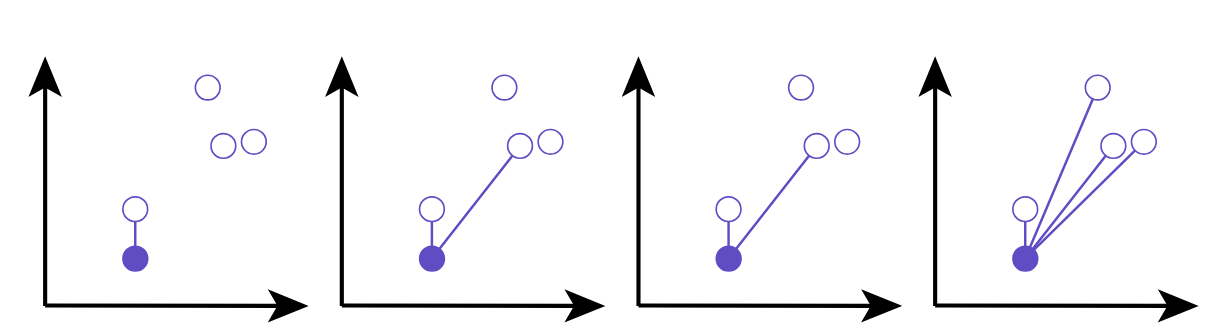
\includegraphics[width=0.9\columnwidth]{images/06/reachneighbors.png}
		\caption{Neighbors at different $k$ values.}
		Local outlier factor respects the postings matrix, as it creates \textit{clusters} of neighbors.
		\label{fig:06/reachneighbors}
	\end{figure}
\end{paracol}


\begin{paracol}{2}
   \colfill
   \textbf{Connectivity outlier factor} is based on the idea that outliers are poorly connected to their neighbors. It is defined as:
   \[
		\tilde{o}(x_i) = \sum_{x_j \in \textit{connect\_neigh}(x_i)} \tilde{o}^k_{i,j}
      \]
      \colfill
   \switchcolumn

   \begin{figure}[htbp]
      \centering
      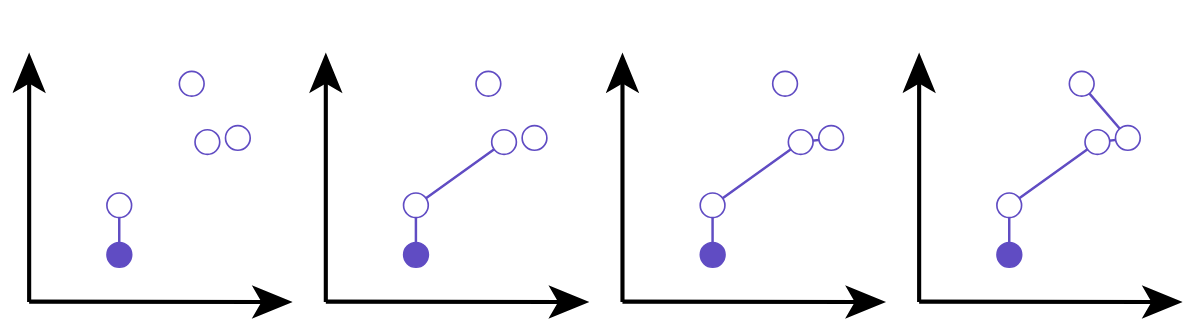
\includegraphics[width=0.95\columnwidth]{images/06/cof.png}
      \caption{Neighbors with different $k$ values.}
      Connectivity Outlier Factor does not respects the posting matrix. Rather, it creates \textit{chains} of neighbors.
      \label{fig:06/cof}
   \end{figure}
\end{paracol}

\begin{paracol}{2}
   \colfill
   \textbf{k-NN} outlier factor (\textsc{kOF}) replaces the average reach at $k$ (denoted with $\bar{\gamma}^k)$ with the maximum reach at $k$ (denoted with $\hat{\gamma}^k$):
   \[
   \tilde{o}(x_i) = \gamma^k(x_i)
   \]
   \colfill
   \switchcolumn

   \begin{figure}[htbp]
      \centering
      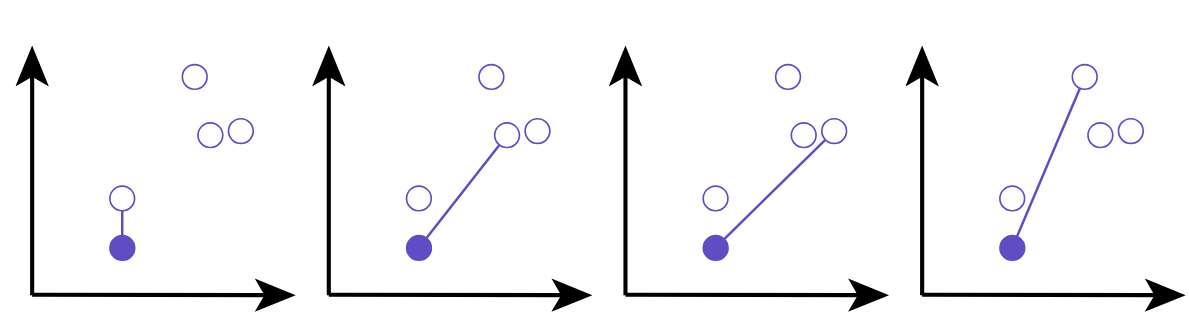
\includegraphics[width=0.95\columnwidth]{images/06/kof.png}
      \caption{Neighbors at different $k$ values}
      \label{fig:06/kof}
   \end{figure}
\end{paracol}

\newpage
\subsection{Concentration}

\begin{paracol}{2}
   We compute concentration on a two-radii approach:
   \begin{itemize}
      \item \textbf{concentration radius} $\varepsilon$: determines the hyperspheres $B(x_i, \varepsilon)$ estimating concentration $c^{\varepsilon}(x_i)$ of $x_i$ within a radius $\varepsilon$
      \item \textbf{neighborhood radius} $\delta$: proportional to $\varepsilon$, determines the neighborhood $B_i$ of $x_i$ as the instances laying within $B(x_i, \delta)$
   \end{itemize}

   \switchcolumn

   \begin{figure}[htbp]
      \centering
      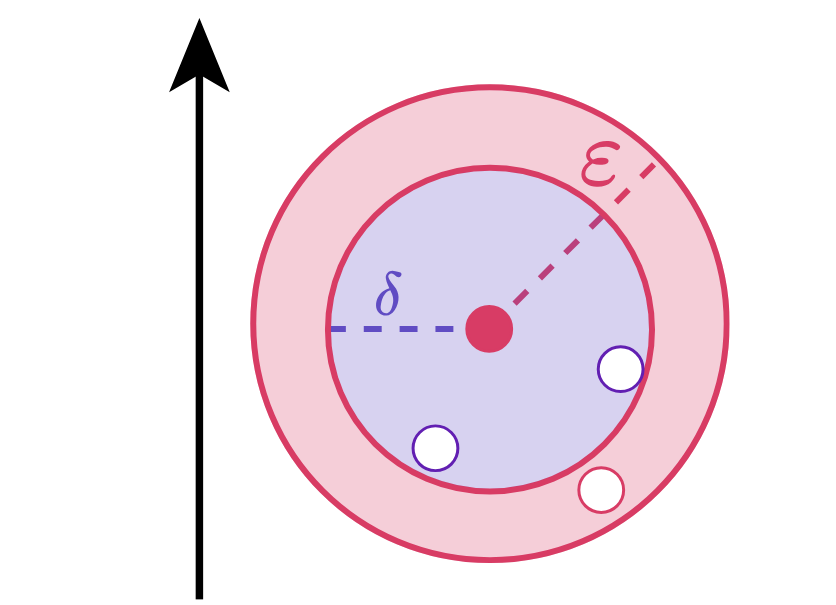
\includegraphics{images/06/tworadii.png}
      \caption{The two radii $\varepsilon, \delta$: the former is used to estimate \textit{concentration}, the latter to choose which neighbors to compare concentration against. \textbf{Note:} $\delta$ may also be larger than $\varepsilon$!}
      \label{fig:06/tworadii}
   \end{figure}
\end{paracol}

\begin{table}[htbp]
   \centering
   \begin{tabular}{|c|c|}
      \hline
      \textbf{Locality} & \textbf{Local} \\
      \hline
      \textbf{Sensitive} & Choice of neighborhood, connectivity parameter \\
      \hline
      \textbf{Interpretable} & Partial: can inspect what instances lead to different reaches\\
      \hline
   \end{tabular}
   \caption{Grading connectivity factors}
   \label{tab:06/connectivity}
\end{table}

\subsection{Neighborhoods}

\begin{figure}[htbp]
   \centering
   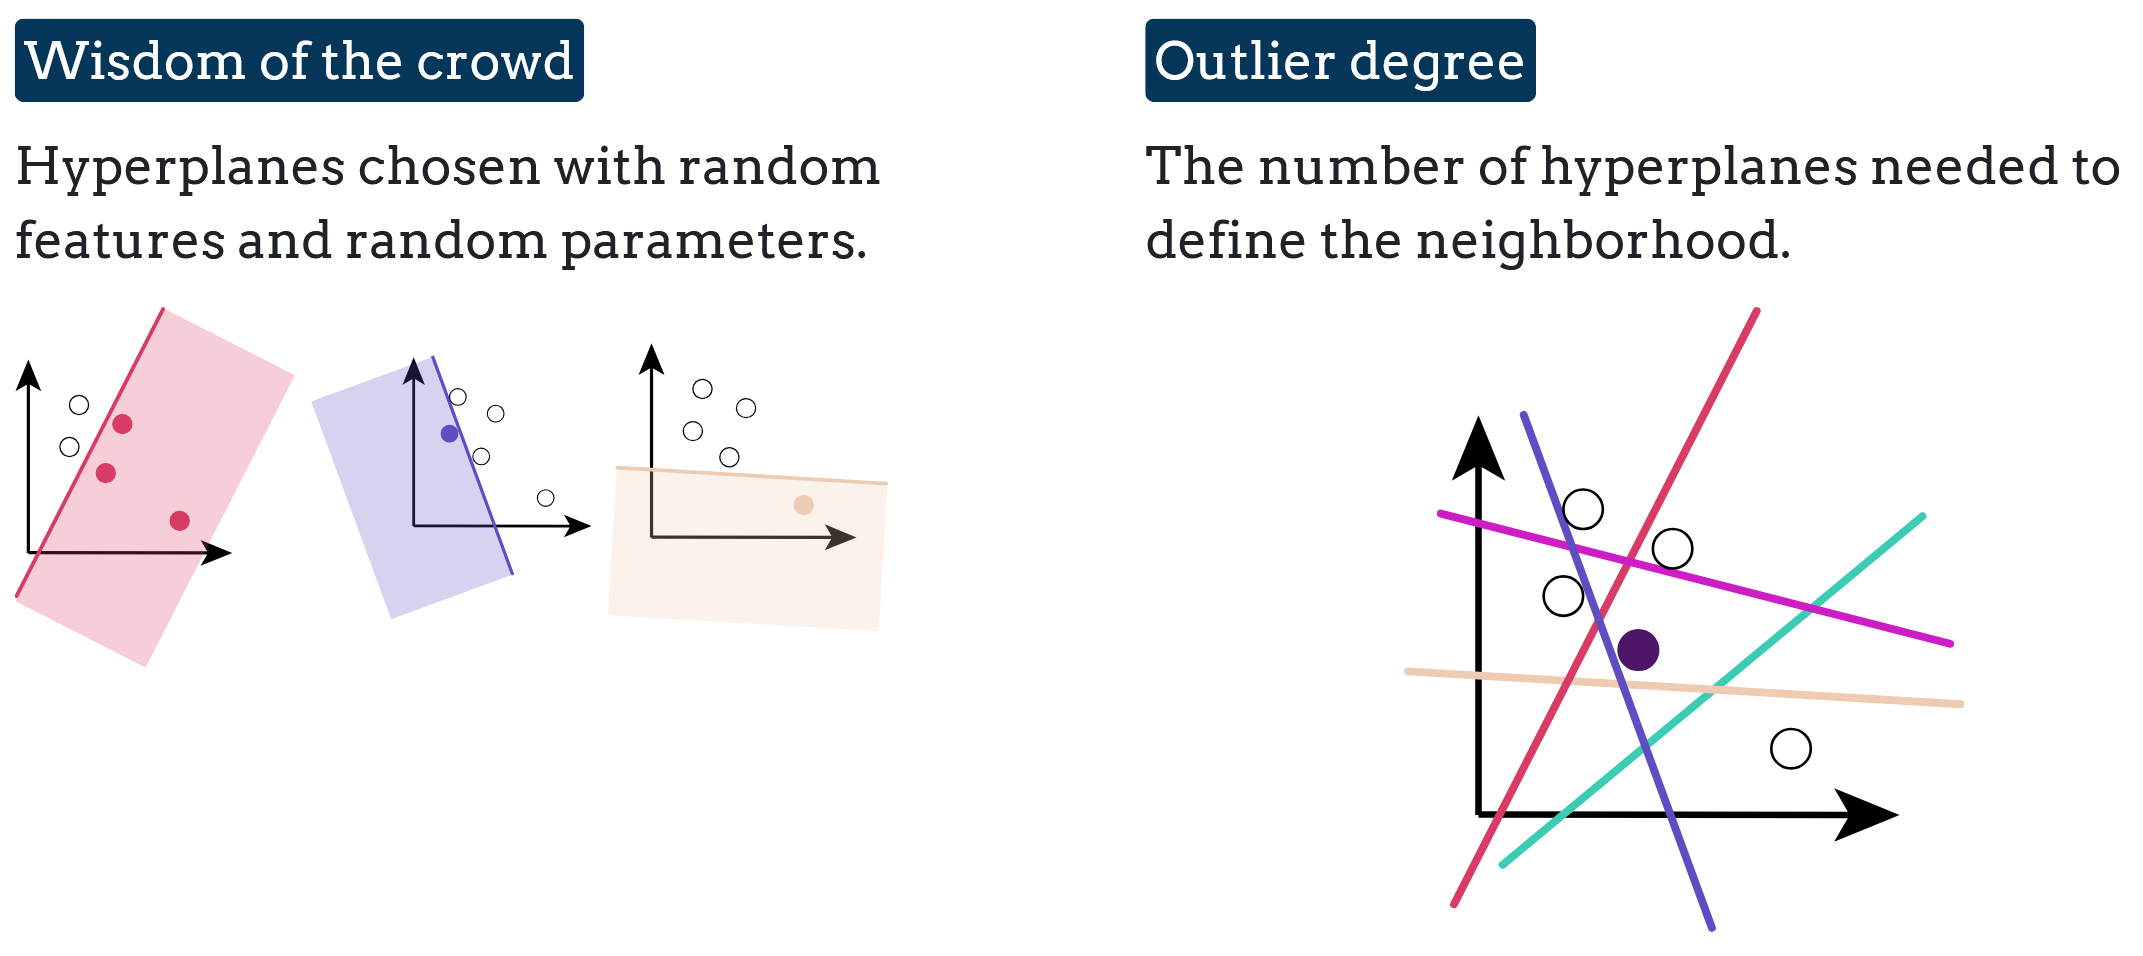
\includegraphics{images/06/hyperplanes.png}
   \caption{Faster and easier to compute hyperplane-based neighborhoods.}
   \label{fig:06/hyperplanes}
\end{figure}

\begin{paracol}{2}
   
   An \textbf{isolation tree} $t$ is a random tree which randomly
   partitions the space into a set of blocks.
   \begin{itemize}
      \item Splits are sampled randomly
      \item Tree grows up to a predefined height, or until all
      leaves contain one instance
   \end{itemize}
   Outlier degree \(\tilde{o}^t(x_i) = \frac{path(x_i,t)}{c} \), where $c$ defines the average path length in the tree.
   
   \switchcolumn

   \begin{figure}[htbp]
      \centering
      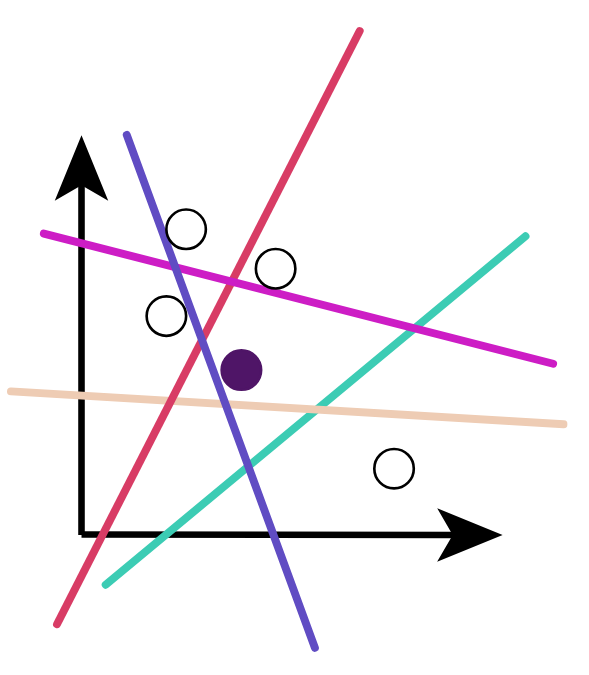
\includegraphics{images/06/isoltree.png}
      \caption{Isolation tree}
      \label{fig:06/isoltree}
   \end{figure}
\end{paracol}

An isolation forest $T$ is comprised of several isolation trees,
further sampling the hyperplane space.
Outlier degree \(\tilde{o}(x_i) = 2 - \frac{\sum_{t \in T} path(x_i,t)}{|T|c}\), where $|T|$ is the number of trees in the forest.

\begin{table}[htbp]
   \centering
   \begin{tabular}{|c|c|}
      \hline
      \textbf{Locality} & \textbf{Global} and \textbf{local} \\
      \hline
      \textbf{Sensitive} & Dataset noise can be interpreted as outlier \\
      \hline
      \textbf{Interpretable} & One of the most interpretable. Splits are induced by the tree, if the tree is univariate. \\
      \hline
      
   \end{tabular}
   \caption{Grading Isolation Forests}
   \label{tab:06/isolation_forests}
\end{table}